\begin{tikzpicture}
	\node[draw, align=center] (problem) at (0, 3){$m=2$\\$n=3$\\$\mathbf{p}=[2,4,5]$\\$D=\varnothing$};

	\draw(2,2) rectangle (4, 4);
	\node[draw, circle] (a) at (2.5, 2.5){};
	\node[draw, circle] (b) at (3, 2.5){};
	\node[draw, circle] (c) at (3.5, 2.5){};
	\node[draw, circle] (d) at (2.5, 3.5){};
	\node[draw, circle] (e) at (3, 3.5){};
	\node[draw, circle] (f) at (3.5, 3.5){};
	\draw[<->] (a) -- (d);
	\draw[<->] (b) -- (e);
	\draw[<->] (c) -- (f);

	\node (chart) at (0, 0){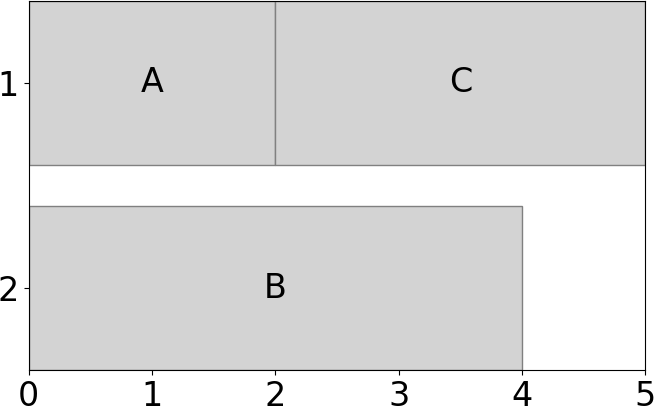
\includegraphics[scale=0.15]{figures/tiny_makespan.png}};
	\node (matrix) at (3, 0){$\begin{bmatrix}
		1 & 0 & 1\\
		0 & 1 & 0\\
		\end{bmatrix}$
	};

	\draw(5,0) rectangle (7, 2);
	\node[draw, circle] (a) at (5.5, 0.5){};
	\node[shaded,draw, circle] (b) at (6, 0.5){};
	\node[draw, circle] (c) at (6.5, 0.5){};
	\node[shaded,draw, circle] (d) at (5.5, 1.5){};
	\node[draw, circle] (e) at (6, 1.5){};
	\node[shaded,draw, circle] (f) at (6.5, 1.5){};
	\draw[<->] (a) -- (d);
	\draw[<->] (b) -- (e);
	\draw[<->] (c) -- (f);
	
	\node[draw](text) at (9, 1){Explanation};
	
	\draw[arrow] (problem) -- (2, 3);
	\draw[arrow] (4, 2.333) -- (5, 1.666);
	\draw[arrow] (chart) -- (matrix);
	\draw[arrow] (matrix) -- (5, 0.666);
	\draw[arrow] (7, 1) -- (text);
\end{tikzpicture}